% !TeX root = ../main.tex
\chapter{合成}\label{ch7}

与预测不同的第二类应用是合成。它包括将密度模型拟合到训练样本上,并提供从该模型中采样的方法。

\section{文本生成}\label{sec7.1}

\keyterm{文本合成}的标准方法是使用基于注意力的\keyterm{自动回归模型}。\cite{Radford2018} 提出了一个非常成功的模型,就是我们在 \ref{sec5.3} 节介绍的 \keyterm{GPT}。

该架构被用于构建超大规模的模型,例如 OpenAI 1750 亿参数的 GPT-3 \citep{arxiv-2005.14165}。它由 96 个自注意力模块构成,每个模块拥有 96 个头,能够处理 12,288 维的 Token,并且在 MLP 中拥有 49,512 隐藏维度。

当该模型在超大规模数据集上训练时,将得到\keyterm{大语言模型}(\keyterm{LLM}),其展现出极其强大的属性。它不仅整合了语言的词法和语法结构,还整合了多种多样的知识,例如预测``日本的首都是''、``如果将水加热到 100 摄氏度将变成''或``Jane 的小狗病了,所以她会''等句子后面的词。

这尤其能够解决\keyterm{小样本预测}问题,即只有少数训练示例可用,如图 \ref{fig7.1} 所示。更令人惊讶的是,当给出精心设计的\keyterm{提示词}时,它可以表现出回答问题、解决问题和思维链的能力,这些能力似乎非常接近高级推理 \citep{arxiv-2204.02311, arxiv-2303.12712}。

\begin{figure}
    \par{\fontsize{9pt}{11pt}
        \hrule
        ~ \\
        I: I love apples, O: positive, I: music is my passion, O: positive, I: my job is boring, O: negative, I: frozen pizzas are awesome, O: \textbf{positive,} \\
        \hrule
        ~ \\
        I: I love apples, O: positive, I: music is my passion, O: positive, I: my job is boring, O: negative, I: frozen pizzas taste like cardboard, O: \textbf{negative,} \\
        \hrule
        ~ \\
        I: water boils at 100 degrees, O: physics, I: the square root of two is irrational, O: mathematics, I: the set of prime numbers is infinite, O: mathematics, I: gravity is proportional to the mass, O: \textbf{physics,} \\
        \hrule
        ~ \\
        I: water boils at 100 degrees, O: physics, I: the square root of two is irrational, O: mathematics, I: the set of prime numbers is infinite, O: mathematics, I: squares are rectangles, O: \textbf{mathematics,} \\
        \hrule
        ~ \\
    }
    \caption[用 GPT 进行小样本预测]{小样本预测示例,采用来自 Hugging Face 的 1.2 亿参数的 GPT 模型。每个示例中,前面的句子是给定的\keyterm{提示词},模型生成的部分用粗体显示。}
    \label{fig7.1}
\end{figure}

由于其卓越的能力,这些模型有时被称为\keyterm{基础模型} \citep{arxiv-2108.07258}。

然而,即便它集成了大量的知识,这样的模型可能仍不足以满足实际应用,特别是在与人类用户交互时。在许多情况下,人们需要根据与助手进行的有效对话的统计数据做出响应。这与现有大规模训练集的统计数据不同,后者结合了小说、百科全书、论坛消息和博客文章。

这种差异可以通过对语言模型进行\keyterm{微调}来解决。目前主流策略是\keyterm{基于人类反馈的强化学习}(\keyterm{RLHF})\citep{arxiv-2203.02155},该策略包括通过要求用户编写回应或对生成的回应进行评分来创建小型标记训练集。前者可以直接用来对语言模型进行微调,而后者可以用来训练一个奖励网络,该网络能够预测评分,并将其作为目标,使用标准的\keyterm{强化学习}方法对语言模型进行微调。

由于语言模型架构大小的急剧增加,训练单一模型的成本可能高达数百万美元(见图 \ref{fig3.7}),因此,微调往往是在特定任务上实现高性能的唯一途径。

\section{图像生成}\label{sec7.2}

已经开发出多种深度方法来对高维密度进行建模和抽样。其中一个用于图像合成的强大方法依赖于反向\keyterm{扩散过程}。

其原理包括分析定义一个逐渐降解任何样本的过程,从而将数据中复杂且未知的密度转化为简单且众所周知的密度,例如正态分布,并训练一个深度架构来反转这一降解过程 \citep{arxiv-2006.11239}。

给定一个固定的 $T$,扩散过程定义了一个关于 $T + 1$ 张图像序列的概率分布,如下所示:从数据集中均匀采样 $x_0$,然后依次采样 $x_{t+1} \sim p(x_{t+1} \mid x_t), t = 0,\dots,T-1$,其中条件分布 $p$ 是分析定义的,并且逐渐擦除了 $x_0$ 中的结构。这种设置应该在很大程度上降解信号,以至于分布 $p(x_T )$ 有一个已知的分析形式,可以进行采样。

\begin{figure}
    \centering
    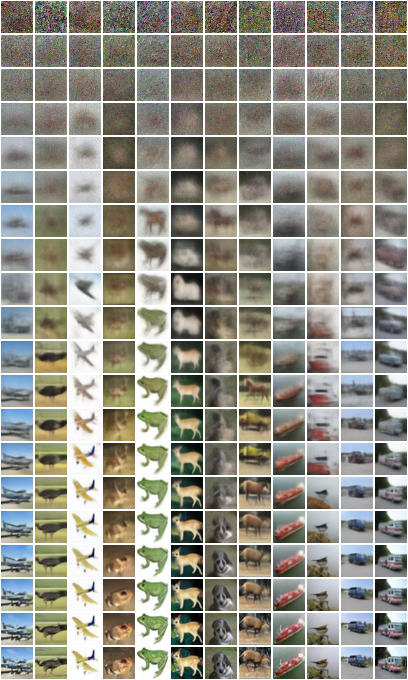
\includegraphics[width=0.9\textwidth]{fig/fig7.2.png}
    \caption[去噪扩散]{用去噪扩散进行图片合成 \citep{arxiv-2006.11239}。每个样本始于白噪音 $x_T$ (顶部),然后分别通过采样 $x_{t-1} \mid x_t \sim \mathcal{N} (x_t + f(x_t,t;w);\sigma_t)$ 逐步去噪。}
    \label{fig7.2}
\end{figure}

例如,\cite{arxiv-2006.11239} 将数据标准化,使其均值为 $0$,方差为 $1$,他们的扩散过程包括添加一点白噪声并将方差重新标准化为 $1$。这一过程指数级减少了 $x_0$ 的重要性,且 $x_t$ 的密度可以迅速用一个正态分布来近似。

去噪器 $f$ 是一个深度架构,其对 $f(x_{t-1},x_t,t;w) \simeq p(x_{t-1} \mid x_t)$ 进行建模并允许从中采样。得益于\keyterm{变分界限},可以证明,如果这个单步反向过程足够准确,那么从 $x_T \sim p(x_T)$ 采样并使用 $f$ 进行 $T$ 步去噪,将得到遵循 $p(x_0)$ 的 $x_0$。

训练 $f$ 可以通过生成大量的序列 $x_0^{(n)}, \dots , x_T^{(n)}$,在每个序列中选取一个 $t_n$,并最大化 
\[\sum_{n} \log f\Big(x_{t_n-1}^{(n)}, x_{t_n}^{(n)}, t_n; w\Big)\]
来实现。

在 \cite{arxiv-2006.11239} 给定的扩散过程中,去噪形式为:
\begin{equation}
    x_{t-1} \mid x_t \sim \mathcal{N} (x_t + f(x_t,t;w);\sigma_t) \label{eq7.1}
\end{equation}
其中 $\sigma_t$ 是以分析方式定义的。

在实践中,这种模型最初通过纯粹的运气在随机噪声中幻想出结构,然后通过强化到目前为止获得的图像最有可能的延续,逐渐构建出从噪声中浮现的更多元素。

这种方法可以扩展到文本条件合成,以生成与描述匹配的图像。例如,\cite{arxiv-2112.10741} 在方程 \ref{eq7.1} 的去噪分布的均值中加入了一个偏差,这个偏差的方向是增加产生的图像与条件文本描述之间的 CLIP 匹配得分(见 \ref{sec6.6} 章)。
